% Synthetic placeholder figure generated from experiment/sec-5-rq3-online-overhead/data/request_latency.csv and pipeline_breakdown.csv
\begin{figure}[t]
  \centering
  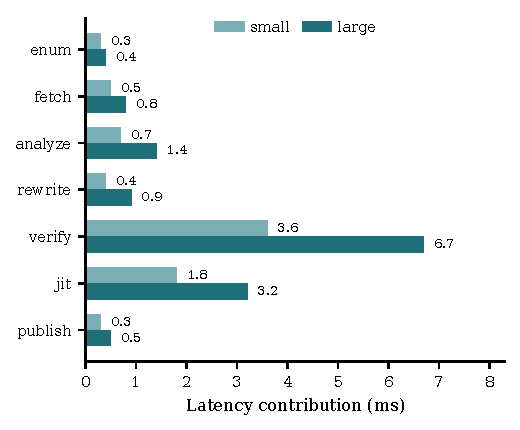
\includegraphics[width=\linewidth]{figures-next/rq3-latency-breakdown.pdf}
  \caption{Per-operation reJIT latency breakdown for small and large targets. In both cases, verifier and JIT dominate the end-to-end cost after request dispatch is amortized. \note{rq-3-exp-1}}
  \label{fig:rq3-latency-breakdown}
\end{figure}
